\documentclass[a4paper,11pt]{article}
\usepackage[utf8]{inputenc}
\usepackage{minted}
\usepackage{amsmath}
\usepackage{float}
\usepackage[symbol]{footmisc}
\usepackage{graphicx}
\usepackage[toc,page]{appendix}

\graphicspath{{./figures/}}
\renewcommand{\thefootnote}{\fnsymbol{footnote}}

\title{\textbf{7. Quicksort}}
\author{Kristiāns Vinters}
\date{Fall 2023}

\begin{document}
    \maketitle
    \section*{Introduction}

    I solved the assignment in Go. I used Go because I want to become more familiar with it. Source code and benchmark data is available on GitHub\footnote[1]{https://github.com/Phanty133/id1021/tree/master/7-quicksort}.

    \section*{Implementation}

    There weren't any particular difficulties in implementing the quicksort algorithms in Go. For the linked list quicksort, I reused the linked list implementation from a previous assignment. The implementations of the quicksort algorithms in Go look very similar to implementations in any other C-like language, with the exception of some Go-specific syntactic sugar, for example, being able to swap variable values in a single line.

    \begin{minted}{go}
func partitionLinkedList(
    min, max *llist.LinkedListItem[int]
) *llist.LinkedListItem[int] {
    // ...
    // Single-line swap example:
    min.Head, max.Head = max.Head, min.Head
    // ...
}
    \end{minted}

    The quicksort implementations for both data types are very similar except for the partition functions. The array partition function has more cases to handle, whereas the linked list function was simpler to implement.

    \begin{minted}{go}
func partitionArray(array []int, min, max int) int {
    pivot := array[min]
    i := min
    j := max

    for i < j {
        for array[i] <= pivot && i < max {
            i++
        }

        for array[j] > pivot && j > min {
            j--
        }

        if i < j {
            array[i], array[j] = array[j], array[i]
        }
    }

    array[min], array[j] = array[j], array[min]

    return j
}

func partitionLinkedList(
    min, max *llist.LinkedListItem[int]
) *llist.LinkedListItem[int] {
	pivot := min
	i := min

	for i != max && i != nil {
		if i.Head < max.Head {
			pivot = min
			i.Head, min.Head = min.Head, i.Head
			min = min.Next()
		}

		i = i.Next()
	}

	min.Head, max.Head = max.Head, min.Head
	return pivot
}
    \end{minted}

    \section*{Benchmarking}

    I benchmarked the sorting algorithms by running them 500 times on different, randomly generated integer arrays for array sizes 10, 100, 1000, 5000, 10000, 50000, 100000, 500000, 1000000. Both implementations were run on the same arrays. I also benchmarked a linked list with a pointer to the last element, but the performance was near identical to the standard linked list, as I access the last element only once in my implementation. For analyzing run times, I measured the raw execution time for every repeat in nanoseconds, which I stored in an array and then wrote to a \texttt{.csv} file. I used LibreOffice Calc to calculate the mean, median, min, and max times and plot the graphs.

    As it turned out, the run times for both the array and linked list implementations were near identical, except that the linked list started to become marginally slower with larger datasets (fig. \ref{fig:ratio}).

    \begin{figure}[H]
        \centering
        
        \begin{tabular}{c|c|c|c}
            Size & $t_\text{Array}$, $\mu s$ & $t_\text{LL}$ & $\frac{t_\text{LL}}{t_\text{Array}}$ \\
            \hline
            \hline
            10 & 1.40 & 1.40 & 1.00 \\
            \hline
            100 & 3.77 & 3.77 & 1.00 \\
            \hline
            1000 & 35.8 & 39.1 & 1.09 \\
            \hline
            5000 & 214 & 239 & 1.12 \\
            \hline
            10000 & 461 & 519 & 1.13 \\
            \hline
            50000 & 2670 & 3060 & 1.15 \\
            \hline
            100000 & 5570 & 6460 & 1.16 \\
            \hline
            500000 & 30700 & 36800 & 1.20 \\
            \hline
            1000000 & 64800 & 78400 & 1.21 \\
        \end{tabular}

        \caption{Median times for array vs linked list quicksort}
    \end{figure}

    \begin{figure}[H]
        \centering
        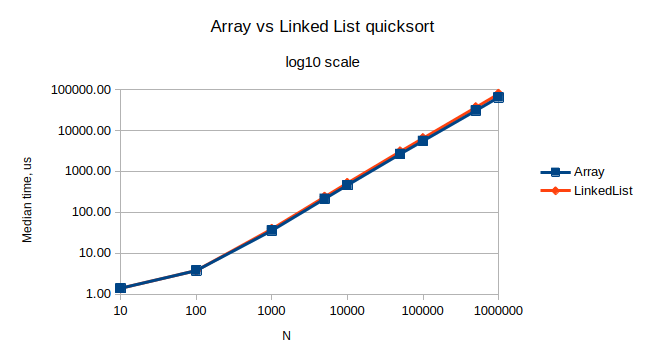
\includegraphics[width=\textwidth]{quicksort.png}
        \caption{Median quick sort times}
        \label{fig:quicksort}
    \end{figure}

    \begin{figure}[H]
        \centering
        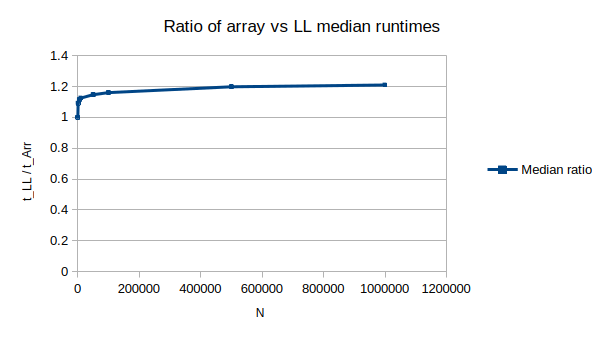
\includegraphics[width=\textwidth]{ratio.png}
        \caption{Median time ratios vs array size}
        \label{fig:ratio}
    \end{figure}

    The expected complexity of quicksort for both the array and linked list (with \texttt{last} pointer) implementation is expected to be $O(n\log_2{n})$. To determine whether my implementations had the same complexity, I plotted the median times against $\text{Array size} * \log_2{\left(\text{Array size}\right)}$ and determined the coefficient of determination $R^2$. $R^2$ was $1.000$ for both (fig. \ref{fig:complexity}).

    \begin{figure}[H]
        \centering
        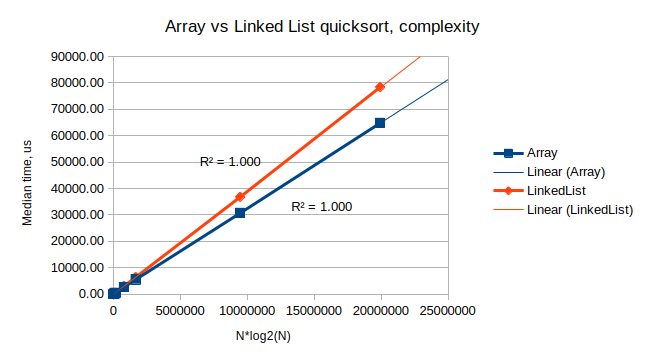
\includegraphics[width=\textwidth]{complexity.png}
        \caption{Implementation time complexity analysis}
        \label{fig:complexity}
    \end{figure}
\end{document}
